% =====================================================================
%  Working paper -- Copies or Colleagues? -- VERSION 1 (November 2026)
%  Version 0 (1 November 2026) is in archive/. The version number stays
%  at 1 until the author decides otherwise.
%  Prose revised with the paper-stil skill on 22 Nov 2026 (content and
%  numbers unchanged; the text before the revision is in archive/).
%  Data: ForecastBench snapshot of 17 Nov 2026 (40 rounds through 2026-10-25).
%  Compile: pdflatex -> bibtex -> pdflatex -> pdflatex
% =====================================================================
\documentclass[11pt,a4paper]{article}

\usepackage[T1]{fontenc}
\usepackage[utf8]{inputenc}
\usepackage{lmodern}
\usepackage{microtype}
\usepackage[margin=1in]{geometry}
\usepackage{setspace}
\usepackage{amsmath,amssymb,amsthm,mathtools}
\usepackage{booktabs,tabularx,array,threeparttable}
\usepackage{ragged2e}
\usepackage{enumitem}
\usepackage[font=small,labelfont=bf]{caption}
\usepackage[round,authoryear]{natbib}
\usepackage{xcolor}
\usepackage{pgfplots}
\usepgfplotslibrary{groupplots}
\pgfplotsset{compat=1.16}
\usepackage[colorlinks=true,linkcolor=blue!50!black,citecolor=blue!50!black,urlcolor=blue!50!black]{hyperref}

\onehalfspacing
\setlist{itemsep=2pt,topsep=4pt}

\newtheorem{proposition}{Proposition}
\theoremstyle{definition}
\newtheorem{hypothesis}{Hypothesis}

\newcolumntype{L}[1]{>{\RaggedRight\arraybackslash}p{#1}}
\newcolumntype{Y}{>{\RaggedRight\arraybackslash}X}
\newcolumntype{C}{>{\centering\arraybackslash}X}

% chart colours (categorical slots 1-3 of the validated reference palette)
\definecolor{cblue}{HTML}{2A78D6}
\definecolor{corange}{HTML}{EB6834}
\definecolor{caqua}{HTML}{1BAF7A}
\definecolor{cink}{HTML}{52514E}

\title{\textbf{Copies or Colleagues?\\Shared Error among AI Models and Human Forecasters}\thanks{Version 1, November 2026. Comments welcome. All data are public (ForecastBench, CC BY-SA 4.0, snapshot of 17 November 2026). The code that produces every number and the data snapshot are available at \url{https://github.com/nikwall/copies-or-colleagues}. Version 0 (1 November 2026) used the snapshot of 31 October 2026. Version 1 adds the round of 25 October 2026, the tournament systems of outside teams (Section~\ref{sec:h7}) and the literature through November 2026. The revision of 22 November 2026 adds a bound on the noise in the outcome (Section~\ref{sec:noise}) and the entries of the teams named in the parity report. I am a founder and managing director of arq decisions, a firm that offers forecasting with human groups. The paper was written with the help of generative AI, and a statement at the end sets out who did what. I thank the ForecastBench team at the Forecasting Research Institute for answering questions about the data. All errors are my own.}}

\author{Niklas Wallmeier\\[2pt]
\small Nieman Foundation at Harvard University and arq decisions\\
\small \href{mailto:niklas.wallmeier@gmail.com}{niklas.wallmeier@gmail.com}}

\date{November 2026}

\begin{document}
\maketitle

\begin{abstract}
\noindent A prominent new account of when AI transforms the economy rests on the premise that a team of people can beat a more capable AI, because people err in different directions while copies of a model do not \citep{imas2026organizing}. I test this premise on ForecastBench, where people and machines forecast the same questions before the outcomes are known, with 578 items answered in 2024 by 500 members of the public, 40 superforecasters and 17 language models, 1.7 million forecasts by 134 models through October 2026, and 647 entries of tool-using systems. Even after removing the largest possible role of noise in the outcome, models from different developers share at least 73 percent of their deviations from the truth with one another, against at least 42 percent among members of the public, and mixing the best models no longer improves on the best one. People kept the lead only where institutions pooled their information, in a team of superforecasters who discussed their forecasts and in prediction markets, whose prices the tool-using systems that reached parity with superforecasters in 2026 match without beating them, which suggests that the human edge in forecasting lies in coordination.
\end{abstract}

\medskip
\noindent JEL codes: C53, D83, J24, L23, O33\\
\noindent Keywords: artificial intelligence, wisdom of crowds, forecast combination, shared error, algorithmic monoculture, prediction markets, organizations

\thispagestyle{empty}
\newpage

% ---------------------------------------------------------------------
\section*{Non-technical summary}
\addcontentsline{toc}{section}{Non-technical summary}
\thispagestyle{empty}

AI models now match experts on many single tasks, yet firms still employ teams of people. One explanation is that people make different mistakes. A team then covers the blind spots of each member, while copies of a model all make the same mistakes. Hence, a team of ordinary people could beat a machine that beats each of them alone. This idea carries a prominent new theory of when AI will transform the economy. But is it true?

Forecasting is one of the few settings where this can be checked, because people and machines answer exactly the same questions before anyone knows the answer. I use a public benchmark with 578 resolved questions from 2024, forecast by 500 members of the public, 40 professional forecasters and 17 AI models, and 1.7 million model forecasts up to October 2026. Starting in late 2025, the benchmark also records systems that outside teams build around the models, with web search, many model calls and averaging. In 2026, such systems caught up with the professional forecasters.

AI models do make the same mistakes. Part of every forecaster's error is the luck of the outcome, which nobody can foresee. Even after taking out as much of that luck as there could be, models from different companies share at least 73 percent of their mistakes, and members of the public at least 42 percent. Combining the five best models used to help a little, and in late 2026 it barely helps. The new tool-using systems are more accurate than plain models, but combining the two adds little. Ordinary people, in contrast, make more varied mistakes, but that variety buys little. On questions about data series, no crowd of laypeople, however large, would have beaten a 2024 model. On questions traded in prediction markets, a handful of laypeople did beat a model, mostly by repeating the market price they had been shown. People stayed ahead where they were organized to pool what they know, in a team of professional forecasters who discussed their forecasts and in the market price itself. Plain models almost never beat that price, and the best tool-using systems now match it by staying close to it.

The human advantage in forecasting therefore seems to come from organization, because markets and teams pool information. That is the capability, coordination, that the theory says AI still lacks. The machines that are catching up are organized too. They are more accurate, but whether they also make different mistakes is too early to tell. For organizations, a group of diverse but unconnected people is weak protection against AI. A well-run market or a team that talks is the benchmark that machines have now reached. A new round of human forecasts, due in 2027, will show whether people are still ahead.

\newpage
\setcounter{page}{1}

% =====================================================================
\section{Introduction}\label{sec:intro}
% =====================================================================

Language models now match or beat experienced professionals on many self-contained tasks. Across 44 occupations, frontier models tie or beat professionals on 48 to 71 percent of bounded deliverables \citep[as summarized by \citealp{imas2026organizing}]{patwardhan2025gdpval}. Yet firms still assign most work to teams of people. \citet{imas2026organizing} explain this gap with an equilibrium model of organizations. Its first building block is that people are jagged in different directions, strong in some domains and weak in others, so a firm can combine them into ``mosaic intelligence''. Copies of a model, in contrast, are jagged in the same direction and add capacity but no breadth. As a result, a team of complementary people can out-compete a model that beats every one of them alone, and the economy may change little until AI learns to coordinate. Forecasting is a case in point. Organizations buy forecasts from crowds, expert teams and prediction markets, and machines are catching up with the best of them. In January 2026, the institute that runs the ForecastBench benchmark wrote: ``If this trend continues, we extrapolate LLM-superforecaster parity in November 2026 (95\% CI: January 2026 -- November 2027)'' \citep{bastani2026closing}. In July 2026, it reported that several systems built by outside teams were statistically indistinguishable from superforecasters \citep{fri2026parity}. But does a crowd of people still add anything that a set of machines cannot supply? On the one hand, people err in different directions, so their errors partly cancel when averaged. Hence, a crowd of weaker people could beat a stronger machine. On the other hand, machines now beat most individuals, and a crowd only helps where the errors of its members are independent. Taken together, it is a priori unclear whether people still add breadth that machines lack. For organizations that pay for forecasts, the answer decides where to spend.

I test the premise where it can be tested directly, on forecasting questions that people and machines answered at the same time, with the same information and before the outcomes were known. I measure how much of each forecaster's error the rest of the group shares, which is the part that averaging cannot remove, and compare individual people with individual models on identical items. The machine side of the premise holds and is getting stronger. Models from different developers share 86 percent of their squared error, almost as much as one model under different prompts (90 percent), while members of the public share 70 percent. Part of this is noise in the outcome, which every forecaster shares. Even after removing the largest possible role of that noise, however, models share at least 73 percent of their deviations from the truth and the public at least 42 percent. Moreover, mixing the best models buys less and less. In the second half of 2026, averaging the five best models improves on the best one by 0.001 Brier points, less than 1 percent. The tool-using systems that caught up with superforecasters are more accurate than the best plain model, by 7 percent for the entries of the three teams named in the parity report, but averaging them with it adds little. The human side holds only in part. People are more diverse, but their crowd beat the 2024 models only on market questions, and there it mostly repeated the market price it had been shown. People kept the lead where institutions pooled their information, in a team of superforecasters who discussed their forecasts and in the prediction market itself. In forecasting, the human edge is therefore coordination, not diversity of minds.

The paper contributes to three strands of research. First, it gives the first direct test of the premise behind the regimes of \citet{imas2026organizing}, and of the older claim that diversity can beat ability \citep{hong2004groups,lamberson2012optimal}, in a setting where both sides answer the same questions. Second, it adds individual human forecasters and tool-using systems to the evidence on correlated errors of AI models. The study closest to this paper is \citet{jeddi2026crowdsourced}, who correlate model errors with human \emph{aggregates} on ForecastBench and find that the correlation rises with model accuracy. \citet{kim2025correlated} show that models err alike on benchmarks without a human comparison, and \citet{spiro2026oracle}, \citet{aitchison2026diversity} and \citet{begin2026preference} document correlated errors among forecasting models and agents. I compare individuals with individuals in one metric and follow the similarity of models over two years without look-ahead in the choice of models. I show that the rise in similarity runs through accuracy and not through time, and I bound how much of the shared error is noise in the outcome, which correlations alone cannot separate from shared mistakes. Third, the paper connects these results to forecast combination \citep{bates1969combination,clemen1989combining} and to the evidence that teaming and markets improve forecasts \citep{mellers2014psychological,wolfers2004prediction,atanasov2017distilling}. A simple model maps the floor of a crowd, the crowd size needed to beat a model and the optimal weight on humans into the regimes of \citet{imas2026organizing}.

Forecasting has two advantages for the question at hand. First, people and machines answer identical questions under identical rules, so their errors can be compared item by item. Second, the questions resolve within days or months, so every forecaster is scored on outcomes that nobody knew at the time. The data come from ForecastBench \citep{karger2025forecastbench}. I use the individual forecasts of its 2024 human round, the forecasts of all models that ForecastBench itself ran in 40 rounds from July 2024 to October 2026, and 647 entries by outside teams since October 2025. The analysis is descriptive measurement on a prospective benchmark. It uses a variance-components split of squared errors, cross-fitted combination weights and a bootstrap that resamples questions. The scope is narrow by design. Forecasting tests the mosaic and competence premises of \citet{imas2026organizing}, but it says nothing about their coordination thesis for AI firms or their results on firm size. Moreover, the only human round with released individual forecasts is from 2024. The comparison of people with the machines of 2026 has to wait for the release of the October 2026 human round.

% =====================================================================
\section{Related literature}\label{sec:literature}
% =====================================================================

Table~\ref{tab:lit} summarizes what prior studies show.

\subsection{Can teams of weaker humans beat a stronger machine?}

\citet{imas2026organizing} model agents with several competences and one coordination capability. A firm's output depends on the mean competence of its members and on how well they coordinate, and complementary humans sort into firms whose mean profile no single member has. Because copies of a model share one profile, a human firm can beat an AI firm whose agents individually beat every human. The authors support this with a quiz in which complementary pairs of people beat random pairs, and with evidence that multi-agent AI systems coordinate poorly. However, they do not test whether models from different developers are as alike as copies, or whether human diversity survives on tasks that both sides perform. The idea has older roots. \citet{hong2004groups} show in a model that a group of diverse problem solvers can beat a group of the best individual solvers. \citet{lamberson2012optimal} show that the best forecasting group trades individual accuracy against the correlation of its members' errors. In team theory, the value of a team depends on how the information of its members combines \citep{marschak1972economic,prat2002homogeneous}. Empirically, groups differ in a collective-intelligence factor that is only weakly related to the individual intelligence of their members \citep{woolley2010evidence}. Task-based models of automation, in contrast, have no such team term. There, a worker's value is set task by task \citep{acemoglu2018race}, and comparative advantage can keep humans employed even when machines are better at every task \citep{restrepo2026wont}.

\subsection{Do machines err alike?}

A literature on algorithmic monoculture asks what happens when many decision makers use the same model \citep{kleinberg2021algorithmic,bommasani2022picking}. For language models, \citet{kim2025correlated} find across more than 350 models that two models agree on the same wrong answer about 60 percent of the time when both err. Models from the same developer and with the same architecture err more alike, and more accurate models err more alike even across developers. In forecasting, \citet{spiro2026oracle} reports an error correlation of 0.77 between three frontier models on 568 questions. \citet{aitchison2026diversity} find on a Metaculus benchmark that the best ensembles combine accurate but less correlated models. The study closest to this paper is \citet{jeddi2026crowdsourced}. They use 76 model-and-prompt sets from 16 models on the same 580 ForecastBench items that I use for 2024, and correlate the errors of each set with those of the superforecaster and public aggregates. The correlation rises with model accuracy by more than independent errors would imply, which they call the accuracy--correlation effect. Because they compare models with human aggregates, however, they cannot say whether individual people are more diverse than individual models. Diversity among machines also seems hard to manufacture. Prompting a model with the behavioral profiles of different traders does not lower the error correlation of an ensemble \citep{qian2026nous}. Preference optimization makes agents in a simulated prediction market err alike, with pairwise correlations near 0.70, and mixing model families is the most effective remedy \citep{begin2026preference}. Across 38 models, pairs that generate their outputs in more different ways fail together less often \citep{tieman2026inferred}. None of these studies compares individual people with individual models, or tool-using systems with the models they are built on.

\subsection{What do humans add to machine forecasts, and how is it pooled?}

Averaging forecasts helps because errors partly cancel \citep{galton1907vox,bates1969combination,clemen1989combining}. How much it helps depends on how much error is shared \citep{davisstober2014crowd}, and shared information biases simple averages \citep{palley2019extracting}. Social influence can make crowds less diverse without making them more accurate \citep{lorenz2011social}. Yet structured interaction can improve accuracy \citep{becker2017network}, and teaming improved accuracy in a large geopolitical tournament \citep{mellers2014psychological}. Prediction markets pool dispersed information through prices \citep{hayek1945use,wolfers2004prediction}, and team-based polls with statistical aggregation can rival them \citep{atanasov2017distilling}. On combining people and machines, an ensemble of 12 models matched a crowd of 925 human forecasters, and averaging human and model forecasts did better still \citep{schoenegger2024wisdom}. A retrieval-based system came close to the human crowd on competition questions \citep{halawi2024approaching}. With tools and scaffolding, machines have since closed much of the remaining gap. A system that combines agentic search, a supervisor agent and statistical calibration matched superforecasters on ForecastBench but stayed below market consensus on liquid markets, and its average with the consensus beat the consensus alone \citep{alur2025aia}. In a study of fifteen models on 254 market questions, the models fell well short of prediction-market accuracy, even after accounting for contamination of their training data \citep{douven2026wisdom}. On ForecastBench itself, superforecasters were ahead of all models in the first rounds \citep{karger2025forecastbench}. By July 2026, several tournament systems were statistically indistinguishable from them, in a comparison that rests on superforecaster forecasts from 2024 adjusted for question difficulty \citep{fri2026parity}. Finally, shared reference points act as shared error in small forecasting crowds \citep{wallmeier2026whom}.

\begin{table}[t]
\centering
\caption{What prior studies show}\label{tab:lit}
\footnotesize
\renewcommand{\arraystretch}{1.12}
\begin{tabularx}{\textwidth}{L{3.3cm} L{4.2cm} Y}
\toprule
Study & Comparison and data & Finding \\
\midrule
\citet{imas2026organizing} & Theory; quiz with 100 people & Complementary humans can beat a better AI; transformation waits for AI coordination \\
\citet{hong2004groups}; \citet{lamberson2012optimal} & Theory & Diversity can beat ability; optimal groups trade accuracy against error correlation \\
\citet{kim2025correlated} & 350+ models on benchmarks; no humans & Models share 60\% of joint errors; more accurate models err more alike \\
\citet{schoenegger2024wisdom} & 12 models vs.\ 925 humans, 31 questions & Model crowd matches human crowd; averaging both helps \\
\citet{karger2025forecastbench} & ForecastBench, 2024 rounds & Superforecasters beat all models \\
\citet{jeddi2026crowdsourced} & 16 models vs.\ human aggregates, 580 items & Model--human error correlation rises with model accuracy \\
\citet{spiro2026oracle} & 3 models, 568 questions & Error correlation 0.77 \\
\citet{aitchison2026diversity} & Models on a Metaculus benchmark & Best ensembles combine accurate but less correlated models \\
\citet{begin2026preference}; \citet{qian2026nous} & Simulated LLM markets; prompted ensembles & Preference optimization creates monoculture; prompts do not add useful diversity \\
\citet{alur2025aia}; \citet{douven2026wisdom} & Tool-using system; 15 models on 254 markets & Systems match superforecasters but not market consensus \\
\citet{fri2026parity} & ForecastBench tournament, 2026 & Tool-using systems statistically tied with 2024 superforecasters \\
\citet{lorenz2011social}; \citet{mellers2014psychological} & Experiments; tournament & Influence reduces diversity; teaming improves accuracy \\
\citet{atanasov2017distilling} & Markets vs.\ polls, tournament & Aggregated team polls can rival markets \\
\midrule
This paper & Individual humans vs.\ individual models on 578 items; 40 rounds of models; 647 tool-using entries & Models err alike beyond outcome noise; tool-using systems are more accurate but add little; human breadth is thin; humans win through markets and teams \\
\bottomrule
\end{tabularx}
\end{table}

% =====================================================================
\section{A simple model}\label{sec:model}
% =====================================================================

\subsection{Set-up}

Forecaster $i$ of type $G\in\{H,M\}$ (human or machine) states a probability $p_{iq}$ for a binary event $q$ with outcome $o_q\in\{0,1\}$. Her error is
\begin{equation}\label{eq:error}
e_{iq}=p_{iq}-o_q=s_{Gq}+u_{iq},
\end{equation}
with a part $s_{Gq}$ shared by all members of her type and an idiosyncratic part $u_{iq}$ with mean zero and variance $\sigma^2_G$, independent across members. The shared part includes the noise in the outcome, which no forecaster can avoid. Write $F_G=\mathbb{E}[s_{Gq}^2]$ for the \emph{floor} of the type and $C=\mathbb{E}[s_{Hq}s_{Mq}]$ for the covariance of the two shared parts. The \emph{shared-error share} $a_G=F_G/(F_G+\sigma^2_G)$ is the part of a member's squared error that averaging cannot remove.

\subsection{Three results}

\begin{proposition}[Crowds and copies]\label{prop:crowd}
The Brier score of the average of $N$ members of type $G$ is $B_G(N)=F_G+\sigma^2_G/N$. Copies of one model have $\sigma^2\approx0$ and add no accuracy. If machine errors are $s_{Mq}=c_q+v_{kq}$ with a common part $c_q$ and a model-specific part $v_{kq}$, the floor of $K$ distinct models is $\mathrm{Var}(c)+\mathrm{Var}(v)/K$. The number of distinct models matters, and the number of copies does not.
\end{proposition}

\begin{proposition}[Weaker members, better crowd]\label{prop:nstar}
Let the best machine score $B_M^*$ and let every human be worse alone, $F_H+\sigma_H^2>B_M^*$. A crowd of humans beats the machine if and only if $F_H<B_M^*$, and then it needs $N^*=\sigma^2_H/(B_M^*-F_H)$ members.
\end{proposition}

\begin{proposition}[Weight on humans]\label{prop:weight}
Combining a human crowd and a machine forecast with weight $w$ on the humans, the weight that minimizes the Brier score at the floors is $w^*=(F_M-C)/(F_H+F_M-2C)$. It is positive if and only if $C<F_M$.
\end{proposition}

Proposition~\ref{prop:nstar} is the forecasting version of mosaic intelligence. A crowd beats a better machine when its shared error is smaller than the total error of the machine. Proposition~\ref{prop:weight} is the optimal combination of \citet{bates1969combination}, and its weight plays the role of the human's bid in \citet{imas2026organizing}. Humans keep a positive weight even next to a better machine, unless the error of the machine is contained in theirs. Moreover, the weight falls as the machine improves while $C$ stays put. Proposition~\ref{prop:crowd} also says what organizing machines can achieve. A system that calls a model several times, averages several models or reconciles their answers removes the model-specific noise $v$. It cannot remove the common part $c$ that all base models share. Only information that the base models lack, such as a market price or fresh news, can move $c$. Hence, a tool-using system that is better than its base models but still errs with them is a better copy and not a colleague. Proofs are in Appendix~\ref{app:proofs}.

\subsection{Regimes}

Table~\ref{tab:regimes} maps the regimes of \citet{imas2026organizing} into this setting. Forecasting has no scale effects, because averaging is a fixed technology without handoffs. Hence, it speaks to competence and mosaic intelligence, but it cannot speak to the coordination of AI firms.

\begin{table}[t]
\centering
\caption{Regimes of \citet{imas2026organizing} in a forecasting task}\label{tab:regimes}
\footnotesize
\renewcommand{\arraystretch}{1.15}
\begin{tabularx}{\textwidth}{L{4.6cm} Y}
\toprule
Regime & Condition \\
\midrule
Weak AI & The best machine is worse than a typical human \\
Minimal AGI & The best machine beats a typical human, but a human crowd beats the machine: $F_H<B_M^*$ \\
Supercompetent, breadth survives & No human crowd beats the machine ($F_H\ge B_M^*$), but humans keep a positive weight ($w^*>0$) \\
Full overlap & $w^*=0$: humans add nothing \\
\bottomrule
\end{tabularx}
\end{table}

\subsection{Hypotheses}

Table~\ref{tab:hyp} states seven hypotheses, each with its test and the result that would falsify it. H1 to H4 follow from \citet{imas2026organizing} and Propositions~\ref{prop:crowd} to \ref{prop:weight}. H5 asks whether the machine side changes as models improve, and H6 asks whether a shared anchor creates shared error. H7 asks whether tool-using systems escape the shared error of their base models. I added H7 in version 1, after the parity report of \citet{fri2026parity}, so its test is exploratory.

\begin{table}[t]
\centering
\caption{Hypotheses, tests and falsifiers}\label{tab:hyp}
\footnotesize
\renewcommand{\arraystretch}{1.15}
\begin{tabularx}{\textwidth}{L{3.8cm} Y Y}
\toprule
Hypothesis & Test & Falsified if \\
\midrule
H1 Copies ladder: one model under different prompts $>$ same developer $>$ different developers $>$ independent humans & Shared-error shares by level, 2024 items & Model levels not above humans \\
H2 Shared jaggedness: $a_M>a_H$ & Distinct models vs.\ the public; question bootstrap & $a_M\le a_H$ \\
H3 Mosaic beats a better machine: $F_H<B_M^*$ & Floors and $N^*$; fixed and best models & $F_H\ge B_M^*$ \\
H4 Breadth survives: $w^*>0$ & Cross-fitted combination weights & $w^*\le0$ \\
H5 Monoculture rises & Shared share of the best models, 39 rounds; models chosen on earlier rounds only & Shared share falls \\
H6 Anchors are shared error & Models with vs.\ without the market price; humans vs.\ the price & No increase in shared error \\
H7 Organized machines are better copies & Tool-using systems vs.\ base models of the same round; systems vs.\ the market price & The best system shares no more error with the best base model than members of the public share with each other ($a\le0.70$), or beats the price consistently \\
\bottomrule
\end{tabularx}
\end{table}

% =====================================================================
\section{Data and identification}\label{sec:data}
% =====================================================================

\subsection{ForecastBench}

ForecastBench \citep{karger2025forecastbench} is a dynamic benchmark that generates binary questions every two weeks and publishes the forecasts and resolutions under a CC BY-SA 4.0 license. Questions come from two sources. \emph{Dataset questions} ask whether a public time series, for example from FRED, ACLED, Yahoo Finance, DBnomics or Wikipedia, will be higher on a resolution date than on the forecast date, at horizons of 7, 30, 90, 180 and 365 days. \emph{Market questions} come from prediction markets and forecasting platforms (Manifold, Metaculus, Polymarket, INFER) and resolve with the event. Each question comes with a ``freeze value'', which is the latest value of the series or the community or market probability on the freeze date. I use the snapshot of the processed forecast sets of 17 November 2026.

\subsection{The 2024 round}

For the round due on 21 July 2024, ForecastBench released individual human forecasts. 500 members of the public, recruited online, answered 20 random questions each in a one-hour survey, which gives about 49 forecasts per item. 40 superforecasters answered over nine days. Halfway through, they saw and discussed each other's forecasts and rationales. Only their final forecasts are released, so I treat them as a communicating team and not as an independent crowd.\footnote{I asked ForecastBench whether the forecasts from before the discussion could be shared. The released file holds one forecast per person and item, with no date or stage field, so the two stages cannot be separated (personal correspondence, November 2026).} The 200 human questions are all part of the 1,000-question set that 17 models answered on the same day, in 128 model-and-prompt versions. The versions differ in the prompt (zero-shot or with a scratchpad, with or without news, and three prompts written by superforecasters) and in whether the model sees the freeze value. People and models were shown the same freeze values, and on all 89 market questions the value is identical in both question sets.\footnote{ForecastBench confirmed that the survey displayed the freeze value to the public and to the superforecasters (personal correspondence, November 2026).} I keep the 578 question-and-horizon items that resolved to 0 or 1 (521 dataset and 57 market items) from 162 questions. I drop 200 public forecasts that lie outside $[0,1]$, which come from respondents who typed a value instead of a probability. The 2.1 percent of model forecasts that ForecastBench imputed are treated as missing.

\subsection{All rounds}

For H5 and H6, I use every model that ForecastBench ran itself with the zero-shot prompt, with and without the freeze value, in 40 rounds from July 2024 to October 2026. This gives 134 models, 7 to 37 per round, and 1.7 million resolved forecasts on single questions. Starting in July 2026, some models forecast with web search, and the main sample excludes those settings. The ``run variants'' in the 2026 rounds are different settings of one model, such as the thinking budget or web search, and not repeated runs. I use the first setting as the model and the others for a comparison within the model.

\subsection{Tournament systems}

Starting in October 2025, ForecastBench also publishes the forecasts of systems that outside teams submit to its tournament. These systems may use tools, retrieval, extra context, fine-tuning or ensembling, and their design is not disclosed. For H7, I use the 647 leaderboard-eligible entries by 101 teams in the 25 rounds from 26 October 2025 to 25 October 2026. An entry enters the comparison of a round if it forecast at least 80 percent of the round's resolved items, which leaves 3 to 114 entries per round. I compare them with the base models of the same round run with the freeze value, which is the closest match to the information that a system can gather.

\subsection{Estimands and estimation}

All Brier scores follow ForecastBench and give the mean over dataset items and the mean over market items equal weight. For a group of forecasters, the squared mean error of an item minus its sampling variance, $\bar e_q^2-\widehat{\mathrm{Var}}_q/n_q$, estimates the squared shared error of the item, and the variance within the item estimates $\sigma^2$. Averaging over items gives $F$, $\sigma^2$ and $a=F/(F+\sigma^2)$. This does not require that two forecasters answer the same items, which the random assignment of the public rules out. Combination weights are cross-fitted in five folds by question. Confidence intervals come from 1,000 bootstrap replicates that resample questions with all their horizons and keep forecasters fixed. For the trend in H5 and the comparisons in H7, I rank the best model, the best system and the top five of each round on earlier rounds only. The ranking uses items that had resolved before the due date of the round and each forecaster's error relative to the item mean of the base models.

\subsection{Validation and limitations}

My scores reproduce ForecastBench's own human medians, exactly for superforecasters (0.122 on dataset and 0.083 on market items) and within 0.002 for the public. The public leaderboard reports difficulty-adjusted scores, which differ from these raw scores. Moreover, the new data snapshot leaves every number for the 2024 round unchanged.

Of course, the approach has limitations. One could argue that people and models did not get the same chance, because people had ten days and models one. However, people saw the freeze values with their questions, so the fair model comparison is the version with the freeze value, which I report alongside the version without it. A second concern is the choice of the best model. Picking the best of 82 model versions without the freeze value, or of 46 with it, after the fact flatters the machines. I therefore also report a model fixed in advance (Claude 3.5 Sonnet with the scratchpad prompt) and select the best version anew in every bootstrap replicate. With up to 114 tournament entries in a round, the concern is larger for H7, which is why I rank the best system on earlier rounds only. A potentially more problematic point is what the shared-error share counts as shared. It includes the noise in the outcome, which no forecaster can avoid, so accurate forecasters may share a large part of their error even when they think independently. For the question whether adding members to a group helps, this is the relevant measure, because averaging cannot remove outcome noise either. But it also means that a high share among accurate forecasters is partly mechanical. Section~\ref{sec:noise} therefore bounds the role of outcome noise from above and reports what remains.

Some things cannot be identified at all. With 20 questions per person, the idiosyncratic error of the public cannot be split into complementary skill and noise. For the superforecaster team, expertise and discussion are confounded. Within a round, comparisons on market items are clean, but which markets have resolved depends on the round, so I do not use market items for trends. Finally, for tournament systems, what a system adds (more model calls, retrieval, a market price or fine-tuning) cannot be separated.

% =====================================================================
\section{Results}\label{sec:results}
% =====================================================================

\subsection{Models err alike (H1, H2)}

Table~\ref{tab:ladder} reports shared-error shares on the 578 items of 2024. Distinct models share 86 percent of their squared error with one another, and frontier models share 92 percent. The 500 independent members of the public share 70 percent, 16 percentage points less than distinct models, and the confidence intervals do not overlap.

\emph{Result 1.} Models err more alike than independent people (supports H2).

The ladder of H1, however, is flat among models. Models from different developers are about as alike as one model under different prompts, and with the scratchpad prompt every model level sits at 0.90 (Appendix Table~\ref{tab:robust}). The pairwise correlation of errors is 0.87 between models and 0.92 between frontier models. This is higher than the 0.77 that \citet{spiro2026oracle} reports for three later models on different questions. One possible reason is the question mix, because data questions with short horizons, which make up most items here, may leave little room for different views. The superforecaster team also has a high share (0.91), but this number says little. Its members are almost as accurate as the best forecast on these items, so the noise in the outcome could explain all of it (Section~\ref{sec:noise}).

\emph{Result 2.} Distinct models are almost as alike as copies of one model (partly rejects H1, whose ladder is flat among models).

\begin{table}[t]
\centering
\caption{Shared-error share by group, 2024 round}\label{tab:ladder}
\footnotesize
\begin{threeparttable}
\begin{tabularx}{0.82\textwidth}{Y r}
\toprule
Group (zero-shot prompt for models) & Shared share $a$ \\
\midrule
Same model, different prompts (mean over 12 models) & 0.90 \\
Different models, same developer (mean over 5 developers) & 0.86 \\
Different developers, one model each & 0.86 \\
All 17 distinct models & 0.86 [0.84, 0.88] \\
Eight frontier models & 0.92 [0.91, 0.93] \\
\addlinespace
Public, independent individuals (500) & 0.70 [0.67, 0.73] \\
Superforecasters after discussion (40) & 0.91 \\
\bottomrule
\end{tabularx}
\begin{tablenotes}\footnotesize
\item \emph{Notes:} $a=F/(F+\sigma^2)$ on 578 items, dataset and market items weighted equally. 95\% intervals from 300 question-level bootstrap replicates. Frontier: Claude 3.5 Sonnet, GPT-4o, Gemini 1.5 Pro, GPT-4 Turbo, Claude 3 Opus, Llama 3 70B, Mistral Large, Qwen 1.5 110B.
\end{tablenotes}
\end{threeparttable}
\end{table}

\subsection{Weaker humans against a better machine (H3)}\label{sec:h3}

84 percent of public individuals score worse than the best model on their own questions. A typical individual scores 0.215, close to the 0.25 of always saying 50 percent. Averaging removes 30 percent of their error and leaves a floor of 0.150. Figure~\ref{fig:crowd} shows what this buys against the models, separately by question type.

\begin{figure}[t]
\centering
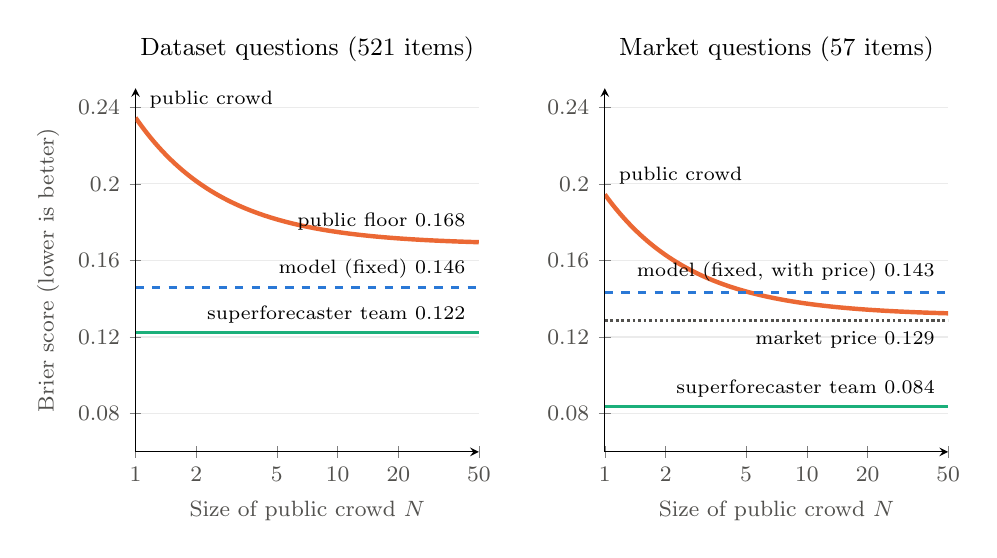
\begin{tikzpicture}
\begin{groupplot}[group style={group size=2 by 1, horizontal sep=1.6cm},
  width=0.49\textwidth, height=6.2cm, xmode=log, xmin=1, xmax=50,
  xtick={1,2,5,10,20,50}, xticklabels={1,2,5,10,20,50},
  ymin=0.06, ymax=0.25, ytick={0.08,0.12,0.16,0.20,0.24},
  yticklabel style={/pgf/number format/fixed,/pgf/number format/precision=2},
  xlabel={Size of public crowd $N$}, axis lines=left,
  tick label style={font=\footnotesize, color=cink}, label style={font=\footnotesize, color=cink},
  title style={font=\small}, ymajorgrids, grid style={black!8}]
\nextgroupplot[title={Dataset questions (521 items)}, ylabel={Brier score (lower is better)}]
  \addplot[corange, line width=1.6pt, domain=1:50, samples=120] {0.1682+0.0664/x};
  \addplot[cblue, line width=1.2pt, dashed, domain=1:50] {0.1458};
  \addplot[caqua, line width=1.2pt, domain=1:50] {0.1223};
  \node[font=\scriptsize, color=black, anchor=south west] at (axis cs:1.05,0.2346) {public crowd};
  \node[font=\scriptsize, color=black, anchor=south east] at (axis cs:48,0.1458) {model (fixed) 0.146};
  \node[font=\scriptsize, color=black, anchor=south east] at (axis cs:48,0.1223) {superforecaster team 0.122};
  \node[font=\scriptsize, color=black, anchor=south east] at (axis cs:48,0.1705) {public floor 0.168};
\nextgroupplot[title={Market questions (57 items)}]
  \addplot[corange, line width=1.6pt, domain=1:50, samples=120] {0.1311+0.0634/x};
  \addplot[cblue, line width=1.2pt, dashed, domain=1:50] {0.1434};
  \addplot[cink, line width=1.0pt, densely dotted, domain=1:50] {0.1286};
  \addplot[caqua, line width=1.2pt, domain=1:50] {0.0836};
  \node[font=\scriptsize, color=black, anchor=south west] at (axis cs:1.05,0.1945) {public crowd};
  \node[font=\scriptsize, color=black, anchor=south east] at (axis cs:48,0.1440) {model (fixed, with price) 0.143};
  \node[font=\scriptsize, color=black, anchor=north east] at (axis cs:48,0.1280) {market price 0.129};
  \node[font=\scriptsize, color=black, anchor=south east] at (axis cs:48,0.0836) {superforecaster team 0.084};
\end{groupplot}
\end{tikzpicture}
\caption{Public crowds against the 2024 models. The orange curve is the expected Brier score of the average of $N$ random members of the public, $F+\sigma^2/N$; resampled crowds match it within 0.001. The dashed line is Claude 3.5 Sonnet with the scratchpad prompt and the freeze value, fixed in advance; the solid line is the superforecaster team; the dotted line is the market price given to everyone.}\label{fig:crowd}
\end{figure}

On \emph{dataset questions}, the public's floor (0.168) lies above the model (0.146), so no crowd of laypeople, however large, beats it. A crowd of laypeople beats the fixed model in only 2 percent of bootstrap replicates, and only the superforecaster team (0.122) beats the model. On \emph{market questions}, a crowd of about five members of the public beats the fixed model even when the model sees the market price ($N^*\approx5$, bootstrap median 6.2, finite in 74 percent of replicates). Prima facie, laypeople beat the AI here. However, this comparison misleads. Against the best model version chosen after the fact (0.129), the crowd wins in only 43 percent of replicates, and the crowd itself is slightly worse than the market price it had been shown (Section~\ref{sec:h6}). Overall, a public crowd beats a model without the price with $N^*\approx7$ (finite in 73 percent of replicates), but it beats the model with the price in only 29 percent. In the language of Table~\ref{tab:regimes}, the 2024 models were supercompetent relative to the public on data questions and at the edge of minimal AGI on market questions. The superforecaster team was ahead on both. Averaging models did not help either, because the crowd of eight frontier models (0.179 overall, zero-shot) scores worse than the best of them.

\emph{Result 3.} A crowd of laypeople beat the 2024 models only on market questions, and there it mostly echoed the price (supports H3 for market questions only).

\subsection{Breadth in a hybrid (H4)}

Table~\ref{tab:hybrid} combines the public crowd with the fixed model. The cross-fitted weight on the public is 0.61 next to the model without the price and 0.39 next to the model with the price, and both intervals exclude zero. Hence, people keep a positive weight even next to a model that beats them, as Proposition~\ref{prop:weight} allows. But the gain from combining, out of sample, is small and cannot be distinguished from zero. The hybrid beats both of its parts in only 44 to 45 percent of replicates. Next to the superforecaster team, the model receives almost no weight ($w^*=0.98$ on the team). At the floors, the shared errors of the public and of the frontier models correlate at 0.93.

\emph{Result 4.} People keep a positive weight next to a better model, but the gain is too small to detect (supports H4 only in its weak form).

\begin{table}[t]
\centering
\caption{Combining the public crowd with a model, 2024 round}\label{tab:hybrid}
\footnotesize
\begin{threeparttable}
\begin{tabularx}{\textwidth}{L{3.6cm} C C C C}
\toprule
 & $w^*$ on public & Hybrid, out of sample & Hybrid minus better part & Hybrid beats both \\
\midrule
Public + fixed model, no price & 0.61 [0.20, 0.94] & 0.148 & $-0.003$ [$-0.006$, $+0.013$] & 45\% \\
Public + fixed model, with price & 0.39 [0.03, 0.73] & 0.142 & $-0.003$ [$-0.005$, $+0.008$] & 44\% \\
\bottomrule
\end{tabularx}
\begin{tablenotes}\footnotesize
\item \emph{Notes:} Public crowd alone 0.151; fixed model 0.159 without and 0.145 with the price. Weights cross-fitted in five folds by question; point estimates averaged over 20 fold splits; 95\% intervals and shares from 1,000 question-level bootstrap replicates.
\end{tablenotes}
\end{threeparttable}
\end{table}

\subsection{Monoculture over two years (H5)}\label{sec:h5}

Table~\ref{tab:h5} and Figure~\ref{fig:h5} follow the models across 39 rounds on dataset questions with horizons of 7 and 30 days, which is the item set that is comparable over time. The last round with resolved 30-day items is that of 11 October 2026. Among the top five models of each round, chosen on earlier rounds only, the shared share rises from 0.96 in the first half of 2025 to 0.97 in 2026, by 0.019 a year ($t=2.6$). Among all models, it is flat. At the level of model pairs, the time trend disappears once accuracy is controlled for. With standard errors clustered by round, the error correlation rises by 0.004 a year (s.e.\ 0.004) and falls by 0.48 per unit of the pair's Brier score (s.e.\ 0.13). More accurate models therefore err more alike, and time adds nothing beyond that. This is the accuracy--correlation effect of \citet{jeddi2026crowdsourced}, traced over two years. Part of it is mechanical, because as forecasts approach the truth, what remains of their errors is the shared noise in the outcome. The bound in Section~\ref{sec:noise} shows that this part is large on these items. Still, net of the largest possible outcome noise, the top five share at least 54 percent of their deviations from the truth. Models from the same developer are slightly more alike (0.006, s.e.\ 0.001). Different settings of one model in 2026 are more alike (0.95 to 0.99) than distinct models in the same round (0.92 to 0.96).

\begin{table}[t]
\centering
\caption{Model monoculture by period, dataset questions with 7- and 30-day horizons}\label{tab:h5}
\footnotesize
\begin{threeparttable}
\begin{tabularx}{\textwidth}{L{1.4cm} C C C C C C C}
\toprule
Period & Rounds & Models (mean) & $a$, all & $a$, top five & Best model & Top-five crowd & Gain from mixing \\
\midrule
2024 & 1 & 17.0 & 0.87 & -- & -- & -- & -- \\
2025 H1 & 9 & 12.2 & 0.95 & 0.96 & 0.166 & 0.162 & $+0.003$ \\
2025 H2 & 8 & 18.5 & 0.92 & 0.93 & 0.171 & 0.164 & $+0.007$ \\
2026 H1 & 13 & 23.2 & 0.93 & 0.97 & 0.161 & 0.158 & $+0.003$ \\
2026 H2 & 8 & 18.6 & 0.94 & 0.97 & 0.171 & 0.170 & $+0.001$ \\
\bottomrule
\end{tabularx}
\begin{tablenotes}\footnotesize
\item \emph{Notes:} Zero-shot prompt without the freeze value; first setting of each model; no web search. ``Best model'' and ``top five'' are ranked on items of earlier rounds that had resolved before the round's due date. Gain: Brier score of the best model minus that of the average of the top five (positive means mixing helps). Robustness checks (7-day items only, prompts with the freeze value, web search included) are in Appendix Table~\ref{tab:robust}.
\end{tablenotes}
\end{threeparttable}
\end{table}

\begin{figure}[t]
\centering
\begin{tikzpicture}
\begin{groupplot}[group style={group size=1 by 2, vertical sep=1.5cm},
  width=0.9\textwidth, height=5.0cm, xmin=2024.45, xmax=2026.85,
  xtick={2024.5,2025,2025.5,2026,2026.5}, xticklabels={Jul 2024,Jan 2025,Jul 2025,Jan 2026,Jul 2026},
  axis lines=left, tick label style={font=\footnotesize, color=cink}, label style={font=\footnotesize, color=cink},
  title style={font=\small}, ymajorgrids, grid style={black!8}, unbounded coords=jump,
  yticklabel style={/pgf/number format/fixed,/pgf/number format/precision=2}]
\nextgroupplot[title={(a) Shared-error share among models}, ymin=0.85, ymax=1.0, ytick={0.85,0.9,0.95,1.0}]
  \addplot[caqua, line width=1.2pt, mark=*, mark size=1.6pt] table[x=t, y=a] {figures/h5_rounds.dat};
  \addplot[cblue, line width=1.6pt, mark=*, mark size=1.8pt] table[x=t, y=a_top] {figures/h5_rounds.dat};
  \node[font=\scriptsize, anchor=south west] at (axis cs:2025.15,0.982) {top five (chosen on earlier rounds)};
  \node[font=\scriptsize, anchor=west] at (axis cs:2024.5,0.862) {all models};
\nextgroupplot[title={(b) Gain from averaging the top five instead of using the best model}, ymin=-0.012, ymax=0.02,
  ytick={-0.01,0,0.01,0.02}, ylabel={Brier points}, scaled y ticks=false,
  yticklabel style={/pgf/number format/fixed,/pgf/number format/precision=2}]
  \addplot[cink, line width=0.8pt, domain=2024.45:2026.85] {0};
  \addplot[cblue, only marks, mark=*, mark size=2.0pt] table[x=t, y=gain] {figures/h5_rounds.dat};
  \node[font=\scriptsize, anchor=south west] at (axis cs:2024.5,0.0005) {above zero: mixing helps};
\end{groupplot}
\end{tikzpicture}
\caption{Models over 39 ForecastBench rounds (dataset questions, 7- and 30-day horizons). Panel (a): shared-error share among all models that ForecastBench ran in a round and among the round's top five. Panel (b): Brier score of the best model minus that of the average of the top five, both ranked on earlier rounds only.}\label{fig:h5}
\end{figure}

The value of breadth among models is small and shrinking. Averaging the top five beats the best model by 0.003 Brier points on average, or 1.8 percent (s.e.\ 0.001), and it wins in 27 of 37 rounds. In the second half of 2026, the gain is 0.001, with wins in 4 of 8 rounds. For comparison, averaging laypeople cut their individual error by 30 percent, and the superforecaster team scored 9 percent below its members.

\emph{Result 5.} The best models grow more alike as they improve, and mixing them no longer pays (supports H5 in the sharper form that monoculture rises with accuracy).

\subsection{The market price as shared error (H6)}\label{sec:h6}

Table~\ref{tab:h6} turns to market questions, where every forecaster received the same market or community probability. Showing models the price pulls their errors toward the error of the price. Within a model, the correlation with the price's error rises by 0.14 in 2024 (all 17 models) and by 0.20 across all rounds, in every round. The distance to the price falls by about 0.14, and the Brier score improves by 0.05 to 0.07. Moreover, the price makes models slightly more alike, as their shared share rises by 0.025 (s.e.\ 0.005). People, who saw the price too, sit close to it. Individual errors correlate at 0.74 with the price's error, and the error of the public crowd at 0.93. The public crowd (0.132) is slightly worse than the price alone (0.129), and an equal average of crowd and price scores 0.125. The superforecaster team (0.084), in contrast, beats the price clearly.

\begin{table}[t]
\centering
\caption{The market price as an anchor}\label{tab:h6}
\footnotesize
\begin{threeparttable}
\begin{tabularx}{\textwidth}{Y c c c c}
\toprule
\multicolumn{5}{l}{\emph{Panel A: 2024 round, 57 resolved market items (price alone: Brier 0.129)}}\\
 & Distance to price & Corr.\ of error with price's error & $a$ & Brier \\
\midrule
Public individuals & 0.179 & 0.74 & 0.67 & 0.192 \\
Superforecasters & 0.128 & 0.80 & 0.87 & 0.093 \\
Models, zero shot, without price & 0.234 & 0.75 & 0.88 & 0.214 \\
Models, zero shot, with price & 0.076 & 0.90 & 0.87 & 0.161 \\
\midrule
\multicolumn{5}{l}{\emph{Panel B: all rounds, within model, price minus no price (670 model-rounds, 101 models)}}\\
 & \multicolumn{2}{c}{Mean change (s.e.\ across 39 rounds)} & \multicolumn{2}{c}{Rounds with this sign} \\
\midrule
Correlation with the market's error & \multicolumn{2}{c}{$+0.20$ (0.009)} & \multicolumn{2}{c}{100\%} \\
Distance to the market price & \multicolumn{2}{c}{$-0.14$ (0.004)} & \multicolumn{2}{c}{100\%} \\
Brier score & \multicolumn{2}{c}{$-0.070$ (0.004)} & \multicolumn{2}{c}{100\%} \\
Shared share among models & \multicolumn{2}{c}{$+0.025$ (0.005)} & \multicolumn{2}{c}{--} \\
\bottomrule
\end{tabularx}
\begin{tablenotes}\footnotesize
\item \emph{Notes:} Panel A uses the freeze value given to humans and models (identical in both question sets). Panel B uses the market price on the due date, a few days after the freeze date; zero-shot prompts; first setting of each model; no web search.
\end{tablenotes}
\end{threeparttable}
\end{table}

The price is hard to beat. Without it, models beat the market price in 1.0 percent of model-rounds, and with it in 5.8 percent. The best model of each round, chosen on earlier rounds, stays behind the price even with the price in its prompt, by 0.011 Brier points since October 2025 (s.e.\ 0.002).

\emph{Result 6.} A shared anchor is a source of shared error for people and machines alike, and here also a source of accuracy that neither the public nor the base models improve on (supports H6).

\subsection{Organized machines (H7)}\label{sec:h7}

Table~\ref{tab:h7} compares the tournament systems with the base models of the same rounds, from October 2025 to October 2026. On dataset questions, the systems are somewhat more diverse than the base models. They share 0.90 of their squared error with one another, against 0.93 among base models. Their errors correlate at 0.93 with the base-model consensus, against 0.97 for a base model with the consensus of the others (difference 0.037, s.e.\ 0.004). The leading system also errs much like the leading base model. Ranked on earlier rounds, the best system and the best base model share 0.93 of their error, and 0.95 in the second half of 2026. However, much of this may be noise in the outcome, because both are close to the best forecast of their round. Net of the largest possible outcome noise, they share at least 40 percent of their deviations from the truth (Section~\ref{sec:noise}). The best system is 2.1 percent more accurate than the best base model (0.162 against 0.166, s.e.\ of the difference 0.003), and it is ahead in 14 of 24 rounds. Averaging the two improves on the system by 0.003 Brier points (s.e.\ 0.001), a gain that vanishes in the second half of 2026. Averaging the top five systems does worse than the best one ($-0.003$, s.e.\ 0.002).

On market questions the change is larger, but it runs through the price. Systems beat the market price in 31 percent of system-rounds, against 6 percent for base models shown the price and 1 percent for base models without it. Their errors correlate at 0.94 with the price's error, more than those of base models shown the price (0.90), and at 0.96 in the second half of 2026. Hence, the systems sit on the price, and many beat it by small margins. The best system chosen on earlier rounds matches the price but does not beat it ($+0.002$ Brier points, s.e.\ 0.002, ahead in 9 of 23 rounds). The best base model with the price, in contrast, stays behind ($+0.011$, s.e.\ 0.002).

The parity report named three teams whose systems were tied with superforecasters: Cassi AI, xAI and Google DeepMind \citep{fri2026parity}. Their 37 entry-rounds in 15 rounds are the parity systems in the narrow sense, and Panel C of Table~\ref{tab:h7} reports them separately. On dataset questions, they are 7 percent more accurate than the best base model of their round (0.152 against 0.164, s.e.\ of the difference 0.003), and they are better in 28 of 37 entry-rounds. Their errors correlate at 0.90 with those of the base model, and averaging the two improves on the entry by only 0.003 Brier points. For these entries, however, the noise bound is weak. They are often the most accurate forecast of their round, so outcome noise could account for nearly all of their shared error (lower bound 0.17). On market questions, they match the price without beating it, with Brier scores 0.000 to 0.005 above the price and error correlations of 0.90 to 0.93 with it.

\emph{Result 7.} The systems that reached parity with superforecasters are more accurate than the base models and sit on the market price, and mixing them with base models adds little. Whether they also make different mistakes, the data cannot show. H7 is not rejected on its stated test. For the parity systems, however, the copy interpretation is not established.

\begin{table}[t]
\centering
\caption{Tournament systems and base models, October 2025 to October 2026}\label{tab:h7}
\footnotesize
\begin{threeparttable}
\begin{tabularx}{\textwidth}{Y c c c}
\toprule
\multicolumn{4}{l}{\emph{Panel A: dataset questions, 7- and 30-day horizons, 25 rounds}}\\
 & \multicolumn{2}{c}{Base models (with freeze value)} & Tournament systems \\
\midrule
Forecasters per round (mean) & \multicolumn{2}{c}{21.4} & 25.5 \\
Shared share among them, $a$ & \multicolumn{2}{c}{0.93} & 0.90 \\
Error correlation with the base-model consensus & \multicolumn{2}{c}{0.97} & 0.93 \\
Brier score of the best, ranked on earlier rounds & \multicolumn{2}{c}{0.166} & 0.162 \\
Best system and best base model: shared share; error correlation & \multicolumn{3}{c}{0.93; 0.94} \\
Gain from averaging the best system with the best base model & \multicolumn{3}{c}{$+0.003$ (0.001); 2026 H2: $0.000$} \\
\midrule
\multicolumn{4}{l}{\emph{Panel B: market questions against the market price, 23 to 27 rounds}}\\
 & Base, no price & Base, with price & Tournament systems \\
\midrule
Share of model-rounds that beat the price & 1.3\% & 6.4\% & 31.4\% \\
Correlation of errors with the price's error & 0.69 & 0.90 & 0.94 \\
Best, ranked on earlier rounds, minus the price & $+0.078$ (0.010) & $+0.011$ (0.002) & $+0.002$ (0.002) \\
\midrule
\multicolumn{4}{l}{\emph{Panel C: entries of the three teams named in the parity report (37 entry-rounds in 15 rounds)}}\\
 & Cassi AI & Google DeepMind & xAI \\
\midrule
Entry-rounds, dataset; market & 6; 9 & 26; 29 & 5; 5 \\
Brier score, entry against best base model & 0.172 vs 0.179 & 0.150 vs 0.163 & 0.138 vs 0.151 \\
Error correlation with the best base model & 0.95 & 0.88 & 0.95 \\
Market: Brier minus price; corr.\ with price's error & $+0.004$; 0.90 & $+0.005$; 0.91 & $+0.000$; 0.93 \\
\bottomrule
\end{tabularx}
\begin{tablenotes}\footnotesize
\item \emph{Notes:} Tournament systems: leaderboard-eligible submissions by outside teams that forecast at least 80\% of a round's items. Base models: models run by ForecastBench, zero-shot prompt with the freeze value, first setting, no web search; the leave-one-out consensus is used for a base model's correlation. Standard errors across rounds in parentheses. Panel B: Brier score relative to the market price on the due date, same items; model-rounds with at least 20 resolved market items (536, 551 and 644). With base models run without the freeze value, the numbers in Panel A change by at most 0.003. Panel C: all entries of Cassi AI, xAI and Google DeepMind with at least 80\% coverage, each compared with the best base model of its round ranked on earlier rounds; market rows use entry-rounds with at least 20 resolved market items.
\end{tablenotes}
\end{threeparttable}
\end{table}

\subsection{How much of the shared error is noise in the outcome?}\label{sec:noise}

The shared-error share counts the noise in the outcome as shared, because no forecaster can avoid it. Two calibrated forecasters therefore share part of their error even when they think independently, and the more accurate they are, the larger this part becomes. Can the gap between models and people be explained this way? Let $U=\mathbb{E}[\pi_q(1-\pi_q)]$ be the irreducible noise, where $\pi_q$ is the probability of event $q$ given everything knowable at the time. Every forecast made at the time has a Brier score of at least $U$. Hence, the lowest Brier score that any forecast achieved on the same items, $B^{\min}$, bounds $U$ from above. If the members of a group were calibrated and erred independently, their floor would be $F=U$, and their shared share could be at most $B^{\min}/B_1$, where $B_1$ is the Brier score of a typical member. The share of each member's deviation from the truth that the group shares is therefore at least $\rho^{LB}=(F-B^{\min})/(F-B^{\min}+\sigma^2)$, or zero if $F\le B^{\min}$. Moreover, the spread $\sigma$, the typical distance of a member's forecast from the group mean in probability points, contains no outcome noise at all.

Table~\ref{tab:noise} reports these measures. In the 2024 round, the lowest Brier score on both question types is that of the superforecaster median (0.103 with equal weights). Independent members of the public could share at most 48 percent of their error, but they share 70 percent, so at least 42 percent of their deviations from the truth are shared. Independent models of the same accuracy could also share at most 48 percent, yet distinct models share 86 percent. Net of the largest possible outcome noise, they share at least 73 percent of their deviations, and frontier models at least 83 percent. Their forecasts also lie closer together, 17 and 12 probability points from the group mean against 25 points for the public. Hence, the gap between models and people survives the bound. For the superforecaster team, in contrast, the bound is uninformative (0.03). Its members are nearly as accurate as the best forecast, so their high share could come from the outcome alone.

On the dataset questions of 2025 and 2026, the bound bites harder. These questions ask whether a series will rise within 7 or 30 days, and many of them are close to a coin flip. The five best models share 96 percent of their error, but independent forecasters of the same accuracy could share up to 89 percent. Net of outcome noise, the top five share at least 54 percent of their deviations, and the best system and the best base model at least 40 percent. For the entries of the parity teams, the lower bound is 0.17. The claim that models err alike therefore rests firmly on the comparison with people in 2024. For the most accurate models and systems of 2026, the data show that mixing them adds little, but they cannot show how much of what remains is shared mistakes and how much is luck.

\begin{table}[t]
\centering
\caption{Shared error net of outcome noise}\label{tab:noise}
\footnotesize
\begin{threeparttable}
\begin{tabularx}{\textwidth}{L{5.6cm} C C C C}
\toprule
 & Shared share $a$ & At most, if independent & At least, net of noise ($\rho^{LB}$) & Spread $\sigma$ \\
\midrule
\multicolumn{5}{l}{\emph{Panel A: 2024 round, 578 items ($B^{\min}=0.103$, superforecaster median)}}\\
Public, independent individuals (500) & 0.70 & 0.48 & 0.42 & 0.25 \\
Superforecasters after discussion (40) & 0.91 & 0.91 & 0.03 & 0.10 \\
All 17 distinct models, zero shot & 0.86 & 0.48 & 0.73 & 0.17 \\
Eight frontier models, zero shot & 0.92 & 0.54 & 0.83 & 0.12 \\
Distinct models, zero shot with freeze value & 0.85 & 0.55 & 0.68 & 0.16 \\
\midrule
\multicolumn{5}{l}{\emph{Panel B: dataset items with 7- and 30-day horizons, 2025 and 2026 ($B^{\min}$ per round)}}\\
Top five models (37 rounds) & 0.96 & 0.89 & 0.54 & 0.08 \\
Best system and best base model (23 rounds) & 0.93 & 0.88 & 0.40 & 0.10 \\
Parity entries and best base model (37 entry-rounds) & 0.90 & 0.90 & 0.17 & 0.12 \\
\bottomrule
\end{tabularx}
\begin{tablenotes}\footnotesize
\item \emph{Notes:} ``At most, if independent'' is $B^{\min}/B_1$, the largest shared share that calibrated members with independent errors and the same accuracy could show. ``At least, net of noise'' is $\rho^{LB}=(F-B^{\min})/(F-B^{\min}+\sigma^2)$. $B^{\min}$ is the lowest Brier score of any forecast with full coverage of the same items: in 2024 the human medians and means, every model version, model means and, on market items, the price (separately by question type, then weighted equally); in later rounds every base model, base-model mean and tournament system. Panel B averages over rounds; the best-system row covers the 23 of 24 rounds of Table~\ref{tab:h7} in which the bound could be computed.
\end{tablenotes}
\end{threeparttable}
\end{table}

% =====================================================================
\section{Discussion}\label{sec:discussion}
% =====================================================================

\subsection{Implications for the theory}

The machine side of the premise of \citet{imas2026organizing} holds, and more strongly than they state it. Distinct models err alike well beyond the noise in the outcome, and mixing them buys less and less as they improve. The human side holds only in a qualified form. Independent people are more diverse, but in forecasting that diversity appears to be largely noise that averaging removes. It did not lift a crowd of laypeople above a 2024 model on data questions, and on market questions it added little to the price that the crowd was given. Where people kept the lead, they did so through institutions that pool information. One is the market, whose price base models rarely beat. The other is a team of experts who discussed their forecasts and stayed more accurate than every model. Both are forms of coordination, the capability that \citet{imas2026organizing} identify as what AI lacks. Hence, the results support their coordination thesis from the human side. They move the human edge from being jagged in different directions to being organized to pool information.

Another interpretation is possible for the superforecaster team. Its lead could come from expertise alone, and the discussion may have added little. The released data cannot separate the two, because the forecasts from before the discussion are not identified. The lead of the team is in line with the evidence that teaming helps \citep{mellers2014psychological}. However, these data cannot show whether the discussion also made the team less diverse, as influence can do in other crowds \citep{lorenz2011social}.

The machines that caught up in 2026 are organized too, because tool-using systems combine model calls and draw on prices and news. They are more accurate than their base models, and on market questions they sit on the price. In the language of Proposition~\ref{prop:crowd}, they may shrink the model-specific error and borrow the information of the market. Whether they also escape the common error of their base models, the data cannot show, because on these questions much of the remaining error may be noise in the outcome. So far, organizing machines has measurably improved their competence, and any gain in breadth is too small to detect.

\subsection{Implications for organizations}

For organizations that buy forecasts, the implications depend on the question. Where a liquid market exists, its price is the benchmark. Base models shown the price stayed behind it through October 2026, and the best tool-using systems matched it. Because the best systems now sit on the price and share their errors with it, a system and a market are not two independent opinions, and averaging them likely buys little. Where no market exists, a trained team that discusses its forecasts was the strongest forecaster in 2024. A crowd of diverse but unconnected people is weak protection against AI. It earns a positive weight in a blend, but the gain is hard to detect. Finally, renting several frontier models instead of the best one no longer pays, and averaging several tool-using systems does worse than picking the best one.

% =====================================================================
\section{Conclusion}\label{sec:conclusion}
% =====================================================================

On questions that people and machines answered at the same time, models from different developers make nearly the same mistakes, and they converge as they improve. Systems that wrap the models in tools are more accurate, and adding them to the models buys little. Ordinary people make more varied mistakes, but their variety is thin protection. In 2024, it beat the models only where it echoed a market price. The human advantage that remained came from markets and teams that pool what people know, and by late 2026 the best machines had reached that benchmark by joining it.

Of course, the evidence comes from one task. Forecasting has no scale effects, so the results say nothing about the coordination of AI agents inside firms or about firm size, which are the core of \citet{imas2026organizing}. Moreover, the only human round with released individual forecasts is from 2024 and is matched against 2024 models. The outside teams do not disclose their designs, so I cannot say whether more model calls, retrieval or the market price drive their gains. The bound on outcome noise is only a bound, and for the most accurate systems it cannot separate shared mistakes from luck. The public answered only 20 questions each, so its diversity cannot be split into skill and noise.

The next test is concrete. ForecastBench ran a second human round in October 2026 and plans to release the individual forecasts under a license agreement, probably in early 2027. With those data, the same measures can show whether the superforecaster team still leads current models and tool-using systems, and whether its lead comes from the discussion. If AI transformation waits for machines to coordinate, as \citet{imas2026organizing} argue, forecasting shows what machines are up against: not diverse individuals, but organized ones.

% =====================================================================
\section*{Statement on the use of generative AI}
% =====================================================================

The research question, the choice of the paper to engage with and the decisions at each stage are mine. Claude (Anthropic) proposed the specific test, wrote the code, downloaded and processed the data, ran the analyses, searched and checked the literature, and drafted the text under my direction, for version 0 and for the update to version 1. Claude then revised the prose of version 1 against a profile of my own writing from before generative AI. Every number in the paper comes from code that reads the public data. I checked the design, the results and the text, and I am responsible for them.

\bibliographystyle{agsm}
\bibliography{references}

\appendix

% =====================================================================
\section{Proofs}\label{app:proofs}
% =====================================================================

\emph{Proof of Proposition~\ref{prop:crowd}.} The average error of $N$ members is $s_{Gq}+\bar u_q$ with $\mathbb{E}[\bar u_q]=0$ and $\mathrm{Var}(\bar u_q)=\sigma^2_G/N$, independent of $s_{Gq}$; its expected square is $F_G+\sigma^2_G/N$. With $s_{Mq}=c_q+v_{kq}$ and $v_{kq}$ independent across models with mean zero, the shared part of the average of $K$ distinct models is $c_q+\bar v_q$ with $\mathbb{E}[(c_q+\bar v_q)^2]=\mathrm{Var}(c)+\mathrm{Var}(v)/K$ when $\mathbb{E}[c_q]=0$; copies share $v_{kq}$ and leave it unchanged. \qed

\emph{Proof of Proposition~\ref{prop:nstar}.} $B_H(N)<B_M^*$ if and only if $F_H+\sigma^2_H/N<B_M^*$. If $F_H\ge B_M^*$ no $N$ satisfies this; otherwise it holds for $N>\sigma^2_H/(B_M^*-F_H)$. \qed

\emph{Proof of Proposition~\ref{prop:weight}.} At the floors, the error of the combination is $ws_{Hq}+(1-w)s_{Mq}$, with expected square $w^2F_H+(1-w)^2F_M+2w(1-w)C$. The first-order condition gives $w^*=(F_M-C)/(F_H+F_M-2C)$; the denominator equals $\mathbb{E}[(s_H-s_M)^2]>0$, so $w^*>0$ if and only if $C<F_M$. \qed

% =====================================================================
\section{Robustness}\label{app:robust}
% =====================================================================

\begin{table}[h]
\centering
\caption{Robustness of H1 and H5}\label{tab:robust}
\footnotesize
\begin{threeparttable}
\begin{tabularx}{\textwidth}{Y c c c c}
\toprule
\multicolumn{5}{l}{\emph{Panel A: shared share by level, 2024 round, scratchpad prompts (items unweighted)}}\\
 & Same developer & One per developer & All models & Frontier \\
\midrule
Scratchpad & 0.90 & 0.90 & 0.90 & 0.93 \\
Scratchpad with freeze value & 0.90 & 0.90 & 0.90 & 0.92 \\
\multicolumn{5}{l}{Same model, different prompts with freeze value: 0.90 (17 models). Public 0.71; superforecasters 0.93.}\\
\midrule
\multicolumn{5}{l}{\emph{Panel B: H5 trends per year (t statistic)}}\\
 & $a$, top five & Corr., top five & Gain from mixing & Pair-level trend \\
\midrule
Main (dataset, 7+30 days) & $+0.019$ (2.6) & $+0.015$ (2.5) & $-0.002$ ($-0.7$) & $+0.004$ (s.e.\ 0.004) \\
7-day items only, all rounds & $+0.018$ (2.9) & $+0.016$ (2.9) & $-0.001$ ($-0.2$) & $+0.004$ (s.e.\ 0.005) \\
With freeze value & $+0.022$ (3.3) & $+0.018$ (3.5) & $+0.000$ ($0.0$) & $+0.004$ (s.e.\ 0.004) \\
Web search included & $+0.017$ (2.3) & $+0.014$ (2.2) & $-0.004$ ($-1.5$) & $-0.000$ (s.e.\ 0.004) \\
\bottomrule
\end{tabularx}
\begin{tablenotes}\footnotesize
\item \emph{Notes:} Panel B: OLS of each round's value on years since July 2024 (HC1 standard errors); pair-level trend from a regression of pair error correlations on time, the pair's Brier score and a same-developer indicator, clustered by round.
\end{tablenotes}
\end{threeparttable}
\end{table}

\end{document}
